% \documentclass[14pt]{extarticle}
\documentclass[bibliography=totocnumbered]{scrartcl}
% \usepackage[english]{babel}
\usepackage[russian]{babel}
\usepackage[utf8x]{inputenc}
\usepackage{amsmath}
\usepackage{graphicx}
\usepackage[colorinlistoftodos]{todonotes}
\usepackage{amssymb}
\usepackage{amsmath}
\usepackage{graphicx}
\usepackage[margin=.8in]{geometry}
\usepackage{listings}
\usepackage[section]{placeins}
\begin{document}

\begin{titlepage}
\newgeometry{margin=2cm}
\newcommand{\HRule}{\rule{\linewidth}{0.5mm}}
\center
\textsc {
\footnotesize{
минобрнауки россии\\
федеральное государственное бюджетное образовательное учреждение\\
высшего профессионального образования}\\
\large{Воронежский государственный университет}
}\\[1.0cm]
\textsc{\largeФакультет компьютерных наук}\\
\textsc{\footnotesizeКафедра информационных технологий}\\[1.0cm] 
\textsc{\Large Эссе}\\[0.5cm]
\HRule \\[0.4cm]
{ \huge \bfseries Системная инженерия на примере системы «Блог»}\\[0.4cm] % Title of your document
\HRule \\[1.5cm]


\begin{flushleft} \large
% \emph{Зав. кафедрой:} Э.К. \textsc{Алгазинов}, д. ф-м н., проф.\\
\emph{Студент:} А.А. \textsc{Валиков} \\
% \emph{Руководитель:} А.В. \textsc{Стромов}, к. ф-м н. % Supervisor's Name
\end{flushleft}

\vfill
\begin{center}
Воронеж 2018
\end{center}
\end{titlepage}

\tableofcontents

\newpage

\section{Введение}

\subsection{Функциональные требования стейкхолдеров}
Блог представляет из себя сайт, посвящённый одному человеку или компании, назовываемыми заказчиком. Для заказчика нужна возможность писать посты, добавлять разделы. Сайт состоит из «админки», -- страницы, на которых заказчик сможет редактировать содержимое сайта и публичиой части.

\paragraph{Заказчик}
\begin{itemize}
    \item Удобство администрирования, то есть структура страниц админки должна быть максимально проста и понятна
    \item Какие части сайта могут быть изменены. После того как сайт сделан, заказчик остаётся один на один с ним, и в случае возникновения новых требований к функционалу, админка можеть позволить (или не дать) добавить новые возможности.
\end{itemize}

\paragraph{Читатели блога}
\begin{itemize}
    \item Современный дизайн
    \item Интуитивно понятные элементы управления (куда тут что нажимать)
    \item Скорость загрузки и работы
    \item Доступность: сайт должен быть доступен максимальное количество времени для максимального количества читателей.
\end{itemize}

\paragraph{Разработчик}
\begin{itemize}
    \item Возможности разработчик отождествляются с возможностями фреймворка, который он использует, поэтому среди технических тербований не должно быть таких, которые невозможно реализовать в этих условиях.
\end{itemize}

Основная функция блога -- \textbf{доставлять информацию от человека, ведущего блог к его читателям}

\subsection{Конструкционные ограничения архитектуры}
Опишем какие основные части составляют блог.
\begin{figure}[htp]
    \centering
    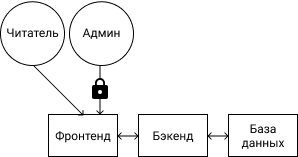
\includegraphics[scale=1.00]{client_server.png}
\end{figure}

\begin{itemize}
    \item \textbf{Фронтенд} -- клиентская часть, открываемая как сайт в браузере пользователя. Фронтенд содержит в себе визуальное отображение страниц, стили, картинка (не все), страницы но без контента.
    \item \textbf{Бэкенд} -- серверная часть, обрабатывающая запросы фронтенда, взаимодействующая для этого с базой данных и  возвращающая клиенту необходимую для работы информацию.
    \item \textbf{База данных} -- более глубокая серверная часть, содержащая динамическую информацию сайта: учётные записи, посты, лайки, комментарии.  
\end{itemize}

\subsection{Описываемая система как холон в иерархии}
Рассмотрим какое место может занять рассматриваемая система как холон в иерархии других холонов -- холархии.
\begin{figure}[!htp]
    \centering 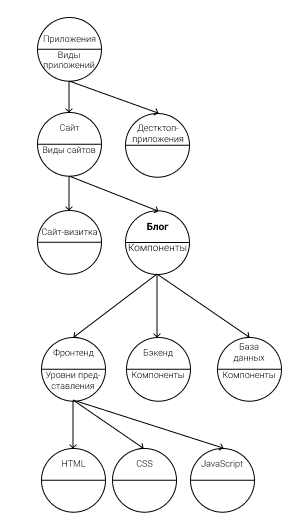
\includegraphics[scale=1]{hol_it.png}
\end{figure}
\subsection{Системы: целевая, обеспечивающая, в эксплуатационной среде}

\paragraph{Целевая система}
Целевой системой будет являться сам блог.

\paragraph{Обеспечивающая система}
\begin{itemize}
    \item Интернет, вероятнее всего с помощью которого будут общаться заказчик и разработчик.
    \item Компьютеры заказчика и разработчика
    \item Разработчик
    \item Фреймворк (то есть программный комплекс, предоставляющий готовые модули для сборки приложения)
    \item Другие необходимые для работы приложения библиотеки
\end{itemize}

\paragraph{Система в эксплуатационной среде}

\begin{itemize}
    \item Серверы, то есть компьютеры, на которых размещён сам сайт либо целиком (фронтенд, бэкенд, база данных), либо частично, тогда используется несколько серверов.

    \item Опять-таки Интернет, но теперь с помощью него содержимое сайта будет доставляться к читателям блога и клиентам. А если фронтенд и бэкенд будут на разных серверах то и для связи между ними.

    \item DNS-сервер, то есть специальная служба позволяющая сопоставить доменное имя (напр. google.com) с IP-адресом фронтенд сервера (именно фронтенд, потому что фронтенд являться точкой входа для клиента)
    
\end{itemize}

Опишем также людей, которым предстоит взаимодействовать с системой, они также будут являться частью системы в эксплуатационной среде:
\begin{itemize}
    \item Клиенты сайта: постоянные читатели блога или люди зашедшие первый раз).
    \item Администратор или модератор (человек, который отвечает только за контент сайта). Их работа, как уже сказано будет производиться в админской части сайта.
\end{itemize}

\section{Жизненный цикл системы согласно V-диаграмме}

\subsection{Определение требований}
На данной стадии происходит сбор и анализ требований к блогу, которые формулируются стейкхолдерами. Требования могут касаться:
\begin{itemize}
    \item Какие разделы желает заказчик видеть доступными для полеьзователя и насколько сайт может быть изменям. Будет ли это конструктор из отдельных виджетов или структура будет жёстко закреплена и потребуется больше времени и навыков для внесения изменений.

    \item Нагрузки на сайт. На какое среднее количество посетителей должна быть расчитана мощность серверов. Здесь же можно отметить отказоустойчивость (сайт должен быть доступен для каждого кто на него зайдёт)

    \item Предполагаемой целевой аудитории. Если блог будет посвящён бизнес-тематике, то вероятно правильнее будет выбрать спокойный, однотонный дизайн без резких акцентов. И, наоборот, если, например, это блог художника-граффтиста, то логично использовать яркие цвета в молодёжном стиле.

    \item Потенциал роста. Если предполагается, что сайт будет расти в дальнейшем и потребуется добавить новый функционал, наприме возможность выкладывать фотографии для фотогралереии, разработчику следует учесть возможное усложнение архитектуры в будущем.
\end{itemize}

\subsection{Архитектурное проектирование}
Решается какие разделы будут на сайте, опеределяются сущности блога (напр. посты, комментарии, фотографии, лайки) и взаимоотношения между ними (посты имеют комментарии, а фотографии лайки).

\subsection{Рабочее проектирование}
Теперь, когда определены разделы и сущности, настаёт времени детальной проработки компонентов. Для фронтенда описывается роутинг, производится разбиение на компоненты. Для бэкенда определяются запросы API. А для базы данных описываются таблицы и взаимоотношения между ними.

\subsection{Изготовление}
Здесь специалисты в своих областях воплощают части блога согласно проекту. Во фронтенде делается вёрстка на HTML, пишутся стили на CSS и описывается логика на JavaScript. Бэкенд-разработчики создают работающее API, таким образом связывая фронтенд и базу данных и они же создают таблицы в базе данных и с помощью внешних ключей описываются взаимоотношения между таблицами. По окончании создания компоненты тестируются специалистами.

\subsection{Интеграция}
Здесь стоит отметить интресную особенность разработки программного обеспечения. Благодаря лёгкости создания, внесения изменений в продукт интеграция может осуществляться в течение всей разработки, с самого её начала (что невозможно в реальном промышленном производстве, где компонент должен быть полностью закончен для того чтобы его можно было интегрировать в ситему). То есть прощё говоря, например, фронтенд-разработчик может сделать одну страницу с одной динамической сущностью, бэкенд описать API на одну сущность и сделать одну таблицу. И уже вот этот очень маленький комплекс может считаться сайтом. То есть как уже было сказано, интеграция производится часто, по мере расширения функционала в частях.

\subsection{Приём в эксплуатацию и эксплуатация}
После окончания внедрения всех функций и исправления ошибок, система проверяется и отдаётся заказчику.

\section{Практики системной инженерии}
В стандарте ISO 15288:2008 указаны 25 обязательных практик системной инженерии. Опишем технические практики, при этом отметим некоторое пересечение с этапами V-диаграммы

\subsection{Сбор требований}
Здесь полностью повторяется пункт «Определение требований» V-диаграммы, то есть в первую очередь заказчик сообщает исполнителю о желаемом функционале.

\subsection{Анализ требований}
При этом исполнитель может посоветовать изменить часть требований по разным причинам (из-за несовместимости, невозможности реализации)

\subsection{Архитектурный дизайн}
Эта практика объединяет в себе этапы «Архитектурное проектирование» и «Рабочее проектирование» V-диаграммы. Можно только добавить, что из-за отностельной лёгкости внесения изменений в проект, проектирование не занимает слишком большого времени (конечно, всё зависит от сложности системы), но чаще всего ограничиваются функционалом, описанием страниц,сущностей, всё это составляет проект и переходят к уже непосредственному воплощению в коде.

\subsection{Изготовление}
Здесь полностью повторяется этап «Изготовление». Добавим, что в разработке ПО как правило используются спринты -- то есть отведённые участки времени (например 2 недели) на которые ставится ряд задач. По окончании спринта проверяется завершённость заданий, если что-то не сделано, оно переходит на следующий спринт. Для каждого разработчика при этом важно проводит своё, так называемое юнит-тестирование, то есть проверка маленьких частей приложения.

\subsection{Интеграция}
То же, что и «Интеграция» в V-диаграмме, -- интеграция происходит с самых ранних этапов разработки, так что не будет пикового момента, когда компоненты долго разрабатывались по отдельности и в короткое время собираются в одну систему.

\subsection{Проверка всей системы}
В разработке ПО этот процесс называется интеграционном тестированием. По мере готовности какого-то логически связанного блока функций, проводится интеграционное тестирование. То есть как и для самой интеграции на весь проект интеграционных тесто может быть достаточно много. Если интеграционный тест выявляет несовпадение с проектом, создаётся задача по исправлению ошибки.

\subsection{Переход к эксплуатации}
По мере изготовления сайт показывается заказчику, после последнего интеграционного теста, может быть объявлено закрытое тестирование среди ограниченного круга пользователей.

\subsection{Валидация}
Выявленные на предыдущем этапе ошибки отправляются на доработку, но обычно на этом этапе не выявляется серьёзных ошибок (конечно при условии хорошее разработки ранее)

\subsection{Эксплуатация}
Система отдаётся заказчику, он получает пароли от сервера, базы данных, собственно админки. Пользователи могут заходить на сайт и читать блог.

\subsection{Обслуживание}

\paragraph{Со строны производителя}
В течение эксплуатации у заказчика могут возникнуть вопросы по системе. Или на этом этапе может быть использован SEO, то есть оптимизация сайта в поисковой выдаче (в идеале если написать "блог" в google то наш сайт должен быть как можно выше)

\paragraph{Со стороны администратора или модератора}
Ведущему блог появляется о чём рассказать, добаляются посты, фотографии. Пользователи делятся и комментируют

\subsection{Вывод из эксплуатации}

Любой сайт живёт пока его смотрят и читают. Если по ряду обстоятельств сайт не набрал и потерял популярность, владелец может решить забрость его. Это будет выражаться отсутствии обновлений, а если владелец перестанет платить за хостинг и домен, то сервер будет очищен и передан другому пользователю как и доменное имя.
\end{document}